% !TeX spellcheck = en_US	

\documentclass[10pt,journal,compsoc]{IEEEtran}
\usepackage{graphicx}
\usepackage[ruled, linesnumbered]{algorithm2e}
\usepackage{url}
\usepackage{epstopdf}
\usepackage{indentfirst}
\usepackage[tight,footnotesize]{subfigure}
\usepackage{amsmath}
\usepackage{amssymb}
\usepackage{multirow}
\usepackage{color}
\usepackage{enumerate}

\newtheorem{theorem}{Theorem}[section]
\newtheorem{lemma}[theorem]{Lemma}
\newtheorem{observation}[theorem]{Observation}
\newtheorem{corollary}[theorem]{Corollary}
\newtheorem{formula}[theorem]{Formula}

% *** CITATION PACKAGES ***
\ifCLASSOPTIONcompsoc
\usepackage[nocompress]{cite}
\else
\usepackage{cite}
\fi

\begin{document}

\title{Building and Checking Suffix and LCP Arrays Using Induced Sorting Method}

\author{Yi~Wu,
	Ge~Nong,
	Wai~Hong~Chan,
	and~Bin~Lao
	\IEEEcompsocitemizethanks{
		\IEEEcompsocthanksitem Y. Wu, G. Nong (corresponding author) and B. Lao are with the Department of Computer Science, Sun Yat-sen University, Guangzhou 510275, China. E-mails: wu.yi.christian@gmail.com, issng@mail.sysu.edu.cn, Laobin@mail3.sysu.edu.cn.
		
		\IEEEcompsocthanksitem Wai Hong Chan (corresponding author) is with the Department of Mathematics and Information Technology, The Education University of Hong Kong, Hong Kong. E-mail: waihchan@ied.edu.hk.
}}% <-this % stops a space


\IEEEtitleabstractindextext{%
\begin{abstract}

<<<<<<< HEAD
Suffix and longest common prefix~(LCP) arrays can be built by the induced sorting~(IS) method on both internal and external memory models. We propose two methods that enable any IS builder to build and check suffix and LCP arrays simultaneously. The first method is for checking both suffix and LCP arrays, while the second method is for checking SA only. By combining the Karp-Rabin fingerprinting techinque into our methods, we design two algorithms that perform checking correctly with a negligible error probability. Theoretically, the algorithm designed by the first method has a sorting complexity, while the algorithm designed by the second method only takes linear time to run. We integrate the algorithm designed by the second method into the existing disk-based suffix sorting algorithm DSA-IS and implement their combination for performance evaluation. From our experiments, the checking overhead is considerably smaller than the building consumption.
=======
Suffix array~(SA) can be built by the induced sorting~(IS) method on both internal and external memory models. We propose two methods that enable any IS suffix sorter to build and check an SA simultaneously. Particularly, the first method checks both suffix and longest common prefix~(LCP) arrays for an input string drawn from a full-ordered alphabet $\Sigma$. By combining our methods with the Karp-Rabin fingerprinting function, we design two algorithms that perform verification with a negligible error probability. Theoretically, the algorithm designed by the first method has a sorting complexity, while the algorithm designed by the second method takes linear time and $\mathcal{O}(\|\Sigma\|)$ RAM space. We integrate the algorithm designed by the second method into the existing suffix sorting algorithm DSA-IS for performance evaluation. Our experiments indicate that the time, space and I/O consumptions for verifcation are considerably smaller than that for construction. We believe that the proposed methods, together with the state-of-the-art IS suffix sorters (and LCP-array builders), could constitute efficient solutions for building and checking suffix (and LCP) array(s) when $\|\Sigma\|$ is much smaller than the size of input string.
>>>>>>> 72e840cf8c9fa565eba557b84e6beb4e2e547367

\end{abstract}

% Note that keywords are not normally used for peerreview papers.
\begin{IEEEkeywords}
Suffix and LCP arrays, construction and verification, internal and external memory.
\end{IEEEkeywords}}


% make the title area
\maketitle

\IEEEdisplaynontitleabstractindextext

\IEEEpeerreviewmaketitle

\section{Introduction}\label{sec:introduction}

<<<<<<< HEAD
A suffix array~(SA) can be built within linear time and space by the internal-memory algorithm SA-IS~\cite{Nong11}. According to the IS principle, the order of two suffixes is determined by comparing their heading characters and successors in sequence, where the order of their successors is assumed to be determined in advance. Recently, the IS method has been also applied to designing three disk-based suffix sorting algorithms eSAIS~\cite{Bingmann12}, DSA-IS~\cite{Nong15} and SAIS-PQ~\cite{Liu15}, where eSAIS can build both suffix and LCP arrays at the same time. These works have better time complexities than the other alternatives ~(e.g., DC3~\cite{Dementiev2008a}, bwt-disk~\cite{Ferragina2012}, SAscan~\cite{Karkkainen2014} and pSAscan~\cite{Karkkainen2015}), but they all suffer from a bottleneck due to the large disk space for obtaining the heading characters of unsorted suffixes and the ranks of their sorted successors in a disk-friendly way. It is reported that the average peak disk use to construct an SA encoded by 40-bit integers for pSAscan is only $7.5n$, while that for eSAIS, DSA-IS and SAIS-PQ are $24n$, $18n$ and $15n$, respectively. The poor space performance of the IS algorithms is mainly because that their current programs fail to free the disk space for temporary data even when the data is no longer to use. A dramatic improvement can be achieved by storing temporary data in multiple files and deleting each file when the data residing on it is not needed any more. This technique has been used to implement a novel IS suffix sorting algorithm fSAIS~\cite{Karkkainen2017}, where the engineering of fSAIS takes no more than $8n$ disk space. This indicates a great potential for optimizing the performances of DSA-IS and SAIS-PQ.

A constructed SA should be checked to detect potential errors caused by implementation bugs and other malfunctions. The software packages for DC3 and eSAIS provide users a checker based on the idea presented in~\cite{Dementiev2008a}. When running on external-memory model, the cost taken by this checker is rather high, because it performs two passes of integer sorts for arranging $\mathcal{O}(n)$ fixed-size tuples. In this paper, we describe two methods that enable any IS builder to build and check suffix and LCP arrays simultaneously. The first method is for checking both suffix and LCP arrays, while the second method is for checking SA only. We employ the Karp-Rabin fingerprinting technique~\cite{Karp1987} to design two probabilistic algorithms, in terms of that their checking results are wrong with a negligible probability. For analysis, we first use new substring sorting and naming methods to improve the design of DSA-IS and then combine the second checking method into the adapted DSA-IS for evaluating the checking overhead. Our experimental results indicate that the time, space and I/O volume for checking SA is considerable smaller than that for building SA. This implies that the IS method can be used to design efficient solutions for SA verification as well.
=======
A suffix array can be built within linear time and space using the internal-memory algorithm SA-IS~\cite{Nong11}. According to the IS principle, the order of two suffixes is determined by sequentially comparing their heading characters and sorted successors. Recently, the IS method has been used to design three disk-based suffix sorting algorithms eSAIS~\cite{Bingmann12}, DSA-IS~\cite{Nong15} and SAIS-PQ~\cite{Liu15}. These works have better time complexities than the other alternatives~(e.g., DC3~\cite{Dementiev2008a}, bwt-disk~\cite{Ferragina2012}, SAscan~\cite{Karkkainen2014} and pSAscan~\cite{Karkkainen2015}), but they suffer from a bottleneck due to the large disk space for obtaining the heading characters of unsorted suffixes and the ranks of their sorted successors in a disk-friendly way. As reported, the average peak disk use to construct an SA encoded by 40-bit integers for eSAIS, DSA-IS and SAIS-PQ are $24n$, $20n$ and $15n$, respectively, while that for pSAScan is only $7.5n$. The poor space performance of the former three algorithms is mainly because that their current programs fail to free the disk space for temporary data even when the data is no longer to use. A dramatic improvement can be achieved by splitting a file into multiple pieces and deleting each piece immediately when the temporary data residing on it is not needed any more. This technique has been used to implement a novel IS suffix sorting algorithm fSAIS~\cite{Karkkainen2017}. The engineering of fSAIS takes no more than $8n$ disk space, indicating a great potential for optimizing the performances of DSA-IS and SAIS-PQ.

A constructed SA should be checked to detect potential errors caused by implementation bugs and hardware malfunctions. The software packages for DC3 and eSAIS provide users a checker that implements the algorithm presented in~\cite{Dementiev2008a}. When running on external-memory model, the checking overhead is rather high because this checker takes two passes of integer sorts for arranging $\mathcal{O}(n)$ fixed-size tuples. In this paper, we describe two methods that enable any IS suffix sorter to build and check an SA at the same time. In particular, the first method is proposed for checking both suffix and LCP arrays. We apply the Karp-Rabin fingerprinting function~\cite{Karp1987} to designing two probabilistic algorithms, in terms of that their checking results are wrong with a negligible probability. We combine the algorithm designed by the second method into DSA-IS and implement the combination to make a performance evaluation, where new substring sorting and naming methods are used to redesign DSA-IS for lowering the peak disk use and I/O volume taken by SA construction. Our experimental results indicate that the time, space and I/O consumptions for verification are negligible to that for construction. This implies that the IS method can be used to design efficient solutions for verification as well.
>>>>>>> 72e840cf8c9fa565eba557b84e6beb4e2e547367

The rest of this paper is organized as follows. Section~\ref{sec:preliminaries} introduces some notations and symbols for presentation convenience. Section~\ref{sec:builder} gives an overview of the existing IS suffix sorting algorithms and show the details of our new substring sorting and naming methods specific for DSA-IS. Section~\ref{sec:checkers} presents the proposed checking methods and the probabilistic algorithms designed by them. Sections~\ref{sec:experiments} and~\ref{sec:conclusion} show the experimental results and the concluding remarks, respectively.

\section{Preliminaries}~\label{sec:preliminaries}

Given a string $x[0,n)$ drawn from a full-ordered alphabet $\Sigma$, we assume the ending character $x[n - 1]$ to be unique and lexicographically smaller than any other characters in $x$. For convenience, we denote by ${\sf suf}(i)$ and ${\sf sub}(i, j)$ the suffix running from $x[i]$ to $x[n-  1]$ and the substring running from $x[i]$ to $x[j]$, respectively. The following notations are also used in our presentation.

<<<<<<< HEAD
Characters in $x$ are classified into two categories: L-type and S-type. We say $x[i]$ is S-type if (1) $i = n - 1$ or (2) $x[i] = x[i + 1]$ and $x[i + 1]$ is S-type; otherwise $x[i]$ is L-type. Further, if $x[i]$ and $x[i - 1]$ are respectively S-type/L-type and L-type/S-type, then $x[i]$ is also called S*-type/L*-type. We use an array $t$ to record the type of all the characters in $x$, where $t[i] = 1$ or $0$ if $x[i]$ is S-type or L-type, respectively. The type of a substring or suffix is determined by that of its heading character.
=======
Characters in $x$ are classified into two categories: L-type and S-type. We say $x[i]$ is S-type if (1) $i = n - 1$ or (2) $x[i] = x[i + 1]$ and $x[i + 1]$ is S-type; otherwise $x[i]$ is L-type. Further, if $x[i]$ and $x[i - 1]$ are respectively S-type/L-type and L-type/S-type, then $x[i]$ is also called S*-type/L*-type. We use an array $t$ to record the type of all the characters in $x$, where $t[i] = 1$ or $0$ if $x[i]$ is S-type or L-type, respectively. A substring or suffix is of the same type as its heading character.
>>>>>>> 72e840cf8c9fa565eba557b84e6beb4e2e547367

Given two characters $x[i]$ and $x[i + 1]$, we say $x[i]$ is the predecessor of $x[i + 1]$ and $x[i + 1]$ is the successor of $x[i]$. We define the predecessor-successor relationship between ${\sf suf}(i)/{\sf sub}(i, j)$ and ${\sf suf}(i + 1)/{\sf sub}(i + 1, j)$.

<<<<<<< HEAD
=======
Partition $x$ into multiple successive S*-type substrings, such that eachsubstring starts with an S*-type character and ends with the leftmost S*-type character on the right side. Produce a reduced string $x_1$ by replacing each S*-type substring with its name, where the name is the rank indicating the lexical order among all.
>>>>>>> 72e840cf8c9fa565eba557b84e6beb4e2e547367

Partition $x$ into multiple S*-type substrings. Each substring only contains two S*-type characters and any two neighboring substrings overlap an S*-type character. Produce a reduced string $x_1$ by replacing each S*-type substring with its name, which represents the rank of the corresponding S*-type substring among all. In the following paragraphs, we use "rank" and "name" interchangeably to indicate the lexical order of the corresponding substring.

The suffix array $sa$ arranges all the suffixes of $x$ in their lexical order, where $sa[i]$ records the starting position of the $(i + 1)$-th smallest suffix. We also define the suffix array $sa_1$ for the reduced string $x_1$ in the same way.

The LCP array $lcp$ records the LCP-value of each pair of neighboring suffixes in $sa$. We assume $lcp[0] = 0$ and let $lcp[i] = \ell$ for $i \in [1, n)$, where $\ell$ is the LCP-value of ${\sf suf}(sa[i])$ and ${\sf suf}(sa[i - 1])$.

All the suffixes in $sa$ are naturally grouped into multiple buckets. Each bucket occupies a contiguous interval in $sa$ and contains all the suffixes with a same heading character. Without loss of generality, we denote by ${\sf sa\_bkt}(c_0)$ the bucket for suffixes starting with $c_0$. It should be noticed that ${\sf sa\_bkt}(c_0)$ can be divided into two parts where the left part ${\sf sa\_bkt_L}(c_0)$ and the right part ${\sf sa\_bkt_S}(c_0)$ contain the L-type and S-type suffixes, respectively. We also define ${\sf lcp\_bkt}(c_0)$, ${\sf lcp\_bkt_L}(c_0)$ and ${\sf lcp\_bkt_S}(c_0)$ on $lcp$ for each character in $\Sigma$.

Let $n_1 = \|x_1\|$, we use $sa^*[0, n_1)$ and $lcp^*[0, n_1)$ to denote the suffix and LCP arrays for S*-type suffixes in $x$, respectively. Specifically, $sa^*[i]$ records the starting position of the $(i + 1)$-th smallest S*-type substring, while $lcp^*[i]$ records the LCP-value of ${\sf suf}(sa^*[i])$ and ${\sf suf}(sa^*[i - 1])$.


\section{Builder}~\label{sec:builder}

\subsection{Introduction to IS Suffix Sorting Algorithms} \label{subsec:improvement}

% Algorithm
\begin{algorithm}
	\SetAlgoNoLine
	\KwIn{$x$}
	\KwOut{$sa$}
	
	/* Reduction Phase */ \\
	Sort S*-type substrings by the IS method. \label{alg:1:ref:1}
	
	Name the sorted S*-type substrings to produce $x_1$. \label{alg:1:ref:2}
	
	~\\
	
	/* Check Recursion Condition */ \\	
	\If{exist two equal characters in $x_1$}{
		
		Recursively call the reduction phase on $x_1$.  \label{alg:1:ref:3}
	}
	\Else{
	
<<<<<<< HEAD
		Compute $sa_1$ from $x_1$.  \label{alg:1:ref:4}
=======
		Compute $sa_1$ from $x_1$.
>>>>>>> 72e840cf8c9fa565eba557b84e6beb4e2e547367
	}
	
	~\\
	
	/* Induction Phase */ \\
	Sort suffixes by the IS method.  \label{alg:1:ref:5}
	
	
	\caption{The Framework of an IS suffix sorting algorithm.}
	
	\label{alg:1}
\end{algorithm}

<<<<<<< HEAD
Algorithm~\ref{alg:1} shows the framework of any IS suffix sorting algorithm. In lines~\ref{alg:1:ref:1}-\ref{alg:1:ref:2}, a reduction phase for sorting and naming S*-type substrings is called to produce the reduced string $x_1$. If there exist duplicate characters in $x_1$, the reduction phase is called with $x_1$ as input at the higher recursion level in line~\ref{alg:1:ref:3}; otherwise, all the S*-type suffixes in $x$ are already sorted and $sa_1$ is directly computed from $x_1$ in line~\ref{alg:1:ref:4}. Afterward, an induction phase for sorting suffixes is called to produce $sa$ for $x$ at the current recursion level in line~\ref{alg:1:ref:5}. The induction phase is recursively called with $sa$ as input at the lower recursion level (if any). 

During the execution of a reduction/induction phase, all the substrings/suffixes are sorted by comparing their heading characters and the ranks of their successors according to the IS principle. This involves a great number of random accesses to $x$ and $sa$, which can be done very fast if both $x$ and $sa$ can wholly reside on RAM. However, if the size of input and output exceeds the capacity of internal memory, each access will take an individual I/O operation, leading to a performance degradation. The DSA-IS algorithm solves the problem by performing the following two steps during a reduction/induction phase:
=======
Algorithm~\ref{alg:1} shows the framework of an IS suffix sorting algorithm. At the very beginning, a reduction phase for sorting and naming S*-type substrings is called to produce the reduced string $x_1$. If there exist duplicate characters in $x_1$, the reduction phase is recursively called with $x_1$ as input; otherwise, all the S*-type suffixes are already sorted and $sa_1$ is directly computed from $x_1$.
Afterward, an induction phase for sorting all the suffixes is called to produce $sa$ for $x$ at current recursion level. The induction phase is recursively called with $sa$ as input until reaching the top recursion level. During the execution of a reduction/induction phase, the order of substrings/suffixes is determined by comparing their heading characters and the ranks of their successors according to the IS principle, which involves a great number of random accesses to $x$ and $sa$. This can be done very fast if both $x$ and $sa$ wholly reside on RAM; otherwise, each access takes an individual I/O operation, leading to a severe performance degradation. This problem is solved in DSA-IS by performing two steps below during the reduction/induction phase:
>>>>>>> 72e840cf8c9fa565eba557b84e6beb4e2e547367

\begin{enumerate}[S1]
	
	\item Split $x$ into blocks and sort substrings/suffixes of each block by calling SA-IS. The heading characters in need are copied to external memory in their access order. \label{dsais_sorting_method:1}
	
	\item Sort the substrings/suffixes by their heading characters and the ranks of their successors in an external-memory heap. Scan the sorted substrings/suffixes in the heap and induce their predecessors into the heap, where the heading characters of the induced substrings/suffixes have been retrieved from external memory in advance by sequential I/O operations. \label{dsais_sorting_method:2}
\end{enumerate}

As shown in Section~\ref{sec:experiments}, our program for DSA-IS requires less disk space than that for eSAIS, but the former runs slower than the latter due to the large I/O volume for sorting and naming S*-type substrings during the reduction phase. To improve the performance, we propose new substring sorting and naming methods in the following.

\subsection{Improvements on DSA-IS}

All the S*-type substrings are classified into long and short categories with respect to whether or not containing more than $D$ characters. The new substring sorting method mainly consists of the three steps below:

\begin{enumerate}[S1']
	\item Sort the long in each block by S\ref{dsais_sorting_method:1}. During the process, copy the short to external memory in their sorted order.~\label{dsaism_sorting_method:1}
	
	\item Sort the long in $x$ by S\ref{dsais_sorting_method:2}. During the process, copy the leftmost $D$ characters of the long to external memory in their sorted order.~\label{dsaism_sorting_method:2}
	
	\item Merge the short and long by a multi-way sorter.~\label{dsaism_sorting_method:3}
\end{enumerate}

<<<<<<< HEAD
After S\ref{dsaism_sorting_method:1}'-S\ref{dsaism_sorting_method:2}', the short S*-type substrings in each block and the long S*-type substrings in $x$ are sorted and separately organized as a sequence in external memory. Assume $x$ is split into $k$ blocks, the multi-way sorter in S\ref{dsaism_sorting_method:3}' maintains an internal-memory heap to cache the current smallest of each sequence and continually retrieve the top item from the heap to determine the lexical order of substrings from different sequences. The heap contains at most $k + 1$ substrings at any point of time and it compares any two substrings in $\mathcal{O}(D)$ time by conducting a literal string comparison\footnote{If the leftmost $D$ characters of a long S*-type substring is equal to a short S*-type substring, then the short is lexicographically greater than the long.}. The above sorting method can achieve a good performance if the majority of S*-type substrings in $x$ are short, provided $D$ is small. This is commonly satisfied in real-world datasets.
=======
After the first two steps, the short S*-type substrings of each block and the long S*-type substrings of $x$ are sorted and separately organized as a sequence in external memory. Assume $x$ is split into $k$ blocks, the multi-way sorter in S\ref{dsaism_sorting_method:3}' maintains an internal-memory heap to cache the current smallest of each sequence and continually retrieves the top item from the heap to determine the lexical order of substrings from different sequences. The heap contains at most $k + 1$ substrings at any point of time and it compares any two substrings in $\mathcal{O}(D)$ time by a literal string comparison\footnote{If the leftmost $D$ characters of a long S*-type substring is equal to a short S*-type substring, then the short is lexicographically greater than the long.}. Theoretically, the sorting method has a good performance if the majority of S*-type substrings in $x$ are short with a small $D$. This is commonly satisfied in practice, because the average length of S*-type substrings is typically small in real-world datasets.

In what follows, we describe a method for naming the S*-type substrings during the above sorting process. The key point here is to check equality of two substrings successively popped from the heap in S\ref{dsaism_sorting_method:3}' as fast as possible. If either of the two substrings is short, we literally compare them in $\mathcal{O}(D)$ time. Otherwise, if both of them are long, then we assign names to all the long S*-type substrings using the technique proposed for SAIS-PQ in S\ref{dsaism_sorting_method:2}' and directly compare two successively popped long S*-type substrings by their names. This technique is based on the idea that two substrings are of the same name if their heading characters and the names of their successors are both equal\footnote{We refer interested readers to~\cite{Liu15} for more information.}.
>>>>>>> 72e840cf8c9fa565eba557b84e6beb4e2e547367

Next, we describe a method for naming the S*-type substrings when they are being sorted. The key point here is to check equality of two substrings successively popped from the heap in S\ref{dsaism_sorting_method:3}' immediately. If either of the two substrings is short, then we literally compare them in $\mathcal{O}(D)$ time to check their equality. Otherwise, the two substrings are both long, we first determine their names when inducing them in S\ref{dsaism_sorting_method:2}' and compare these names in $\mathcal{O}(1)$ time to check their equality. This naming technique was originally proposed for SAIS-PQ for merging the sorting and naming processes into a whole. The experimental results in Section~\ref{sec:experiments} indicate that, by using the new substring sorting and naming methods, the adapted DSA-IS, called DSA-IS+, only takes half as much disk space as eSAIS.

\section{Checkers}~\label{sec:checkers}

\subsection{Prior Art} \label{sec:checkers:prior_art}

We describe below the main idea of the existing checker presented in~\cite{Dementiev2008a}.

\begin{lemma} \label{lemma:1}
	$sa[0, n)$ is the SA for $x[0, n)$ if and only if the following conditions are satisfied:\\
	(1) $sa$ is a permutation of $[0, n)$. \\	
	(2) ${\sf r_i < r_j} \Leftrightarrow (x[i], r_{i + 1}) < (x[i], r_{j + 1})$ for $ i, j \in [0, n)$ and $i\ne j$, where $r_i$ and $r_j$ represent the ranks of ${\sf suf}(i)$ and ${\sf suf}(j)$ among all the suffixes, respectively. \\
\end{lemma}

\begin{IEEEproof}The first condition indicates that $sa$ is a permutation of all the suffixes in $x$. The second condition indicates that the order of suffixes in $sa$ corresponds to that of their heading characters and successors. Because any two suffixes can be sorted by comparing their heading characters and successors, the above conditions are sufficient and necessary for SA verification.

\end{IEEEproof}

The disk-based implementation of this checker conducts two passes of integer sorts and each sort arranges the order of $\mathcal{O}(n)$ fixed-size tuples using external memory. As can be observed from Section~\ref{sec:experiments}, the peak disk use and the I/O volume for an SA encoded by 40-bit integers are around $26n$ and $53n$, respectively.

\subsection{Proposals} \label{sec:checkers:proposals}

<<<<<<< HEAD
Recall that, an IS suffix sorting algorithm recursively perform the reduction phase to compute the reduced string $x_1$ until $x_1$ contains no duplicate characters. Afterward, it produces $sa_1$ from $x_1$ and recursively perform the induction phase to compute $sa$ until reaching the top recursion level, where the induction phase consists of the following steps:
=======
Remember that an IS suffix sorting algorithm recursively performs the reduction phase to compute the reduced string $s_1$ until $s_1$ contains no duplicate characters. Afterward, it produces $sa_1$ from $s_1$ and recursively perform the induction phase to compute $sa$ until reaching the top recursion level, where the induction phase consists of the following steps:
>>>>>>> 72e840cf8c9fa565eba557b84e6beb4e2e547367

\begin{enumerate}[S1'']
	\item sort the starting positions of all the S*-type suffixes with their ranks indicated by $sa_1$ to produce $sa^*$ \label{induction_phase:1}.

	\item Clear $sa$. Scan $sa^*$ leftward with $i$ decreasing from $n_1 - 1$ to $0$. For each scanned item $sa^*[i]$, insert it into the rightmost empty position of ${\sf sa\_bkt_S}(x[sa^*[i]])$. \label{induction_phase:2}
	
	\item Scan $sa$ rightward with $i$ increasing from $0$ to $n - 1$. For each scanned non-empty item $sa[i]$, insert $sa[i] - 1$ into the leftmost empty position of ${\sf sa\_bkt_L}(x[sa[i] - 1])$ if $t[sa[i] - 1] = 0$.\label{induction_phase:3}
	
	\item Clear ${\sf sa\_bkt_S}(c)$ for $c \in \Sigma$. Scan $sa$ leftward with $i$ decreasing from $n - 1$ to $0$. For each scanned non-empty item $sa[i]$, insert $sa[i] - 1$ into the rightmost empty position of ${\sf sa\_bkt_S}(x[sa[i] - 1])$ if $t[sa[i] - 1] = 1$.\label{induction_phase:4}
	
\end{enumerate}

<<<<<<< HEAD
A running example of S\ref{induction_phase:2}''-S\ref{induction_phase:4}'' is shown in Fig.~\ref{fig:example1}. Given $sa^*$ is already known, line 6 inserts each S*-type suffix into the right part of the corresponding bucket and arranges them according to their sorted order indicated by $sa^*$. For example, ${\sf suf}(8)$, ${\sf suf}(5)$, ${\sf suf}(2)$ are placed into the right part of ${\sf sa\_bkt}(i)$ and arranged in their sorted order indicated by $sa^*$. Next, we find the leftmost position of each bucket (marked by the symbol $\wedge$) and scan $sa$ rightward for inducing the order of L-type suffixes. For this, we first check $sa[0] = 14$ (marked by the symbol @) and induce the predecessor of ${\sf suf}(14)$ in lines 8-9. Because $x[13] = i$ is L-type, we put ${\sf suf}(13)$ into the current leftmost empty position in ${\sf sa\_bkt_L}(i)$. To step through $sa$ in this way, we get all the L-type suffixes sorted in line 17. Afterward, we find the rightmost position of each bucket and scan $sa$ leftward for inducing the order of S-type suffixes. When scanning $sa[14] = 4$ in lines 19-20, we see $x[3] = i$ is S-type and thus put ${\sf suf}(3)$ into the current rightmost empty position in ${\sf sa\_bkt_S}(i)$. Following the same idea, we get all the S-type suffixes sorted in line 28. Based on the discussion, we show in Lemma~\ref{lemma:2} a set of sufficient and necessary conditions for SA verification.
=======
A running example of S\ref{induction_phase:2}-S\ref{induction_phase:4} is shown in Fig.~\ref{fig:example1}. Given $sa^*$ is already known, line 6 inserts each S*-type suffix into the right part of the corresponding bucket and arranges them according to their sorted order indicated by $sa^*$. For example, $\sf suf(2)$, $\sf suf(5)$, $\sf suf(8)$ are placed at the rightmost empty position of $\sf sa\_bkt(i)$ in sequence. Then, we find the leftmost position of each bucket (marked by the symbol $\wedge$) and scan $sa$ rightward for inducing the order of L-type suffixes. To do this, we first check $sa[0] = 14$ (marked by the symbol @) and induce the predecessor of $\sf suf(14)$ in lines 8-9. Because $x[13] = i$ is L-type, we put $\sf suf(13)$ into the current leftmost empty position in $\sf sa\_bkt_L(i)$. To step through $sa$ in this way, we get all the L-type suffixes sorted in line 17. Afterward, we find the rightmost position of each bucket and scan $sa$ leftward for inducing the order of S-type suffixes. When scanning $sa[14] = 4$ in lines 19-20, we see $x[3] = i$ is S-type and thus put $\sf suf(3)$ into the current rightmost empty position in $\sf sa\_bkt_S(i)$. Following the same idea, we get all the S-type suffixes sorted in line 28. Based on the discussion, we show in Lemma~\ref{lemma:2} a set of sufficient and necessary conditions for SA verification.
>>>>>>> 72e840cf8c9fa565eba557b84e6beb4e2e547367


\begin{figure}[t]
	\centering
	
	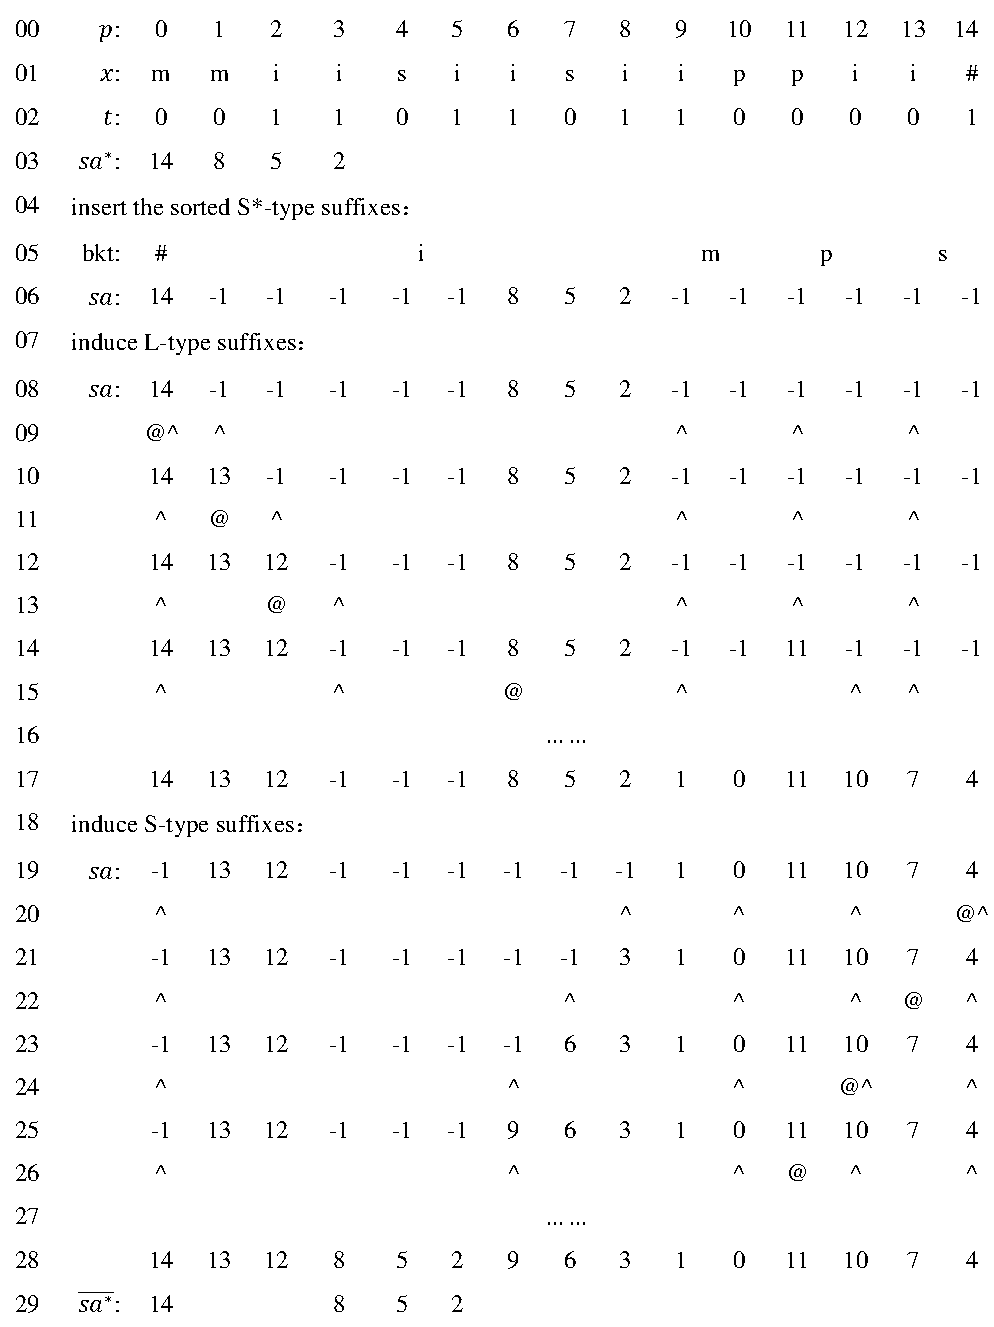
\includegraphics[width = 1\columnwidth]{example.pdf}
	
	\caption{An example for inducing $sa$ from $sa^*$.}
	
	\label{fig:example1}
	
\end{figure}


\begin{lemma} \label{lemma:2}
    $sa[0, n)$ is the SA for $x[0, n)$ if and only if the following conditions are satisfied: \\
    (1) $sa^*$ is correctly computed. \\
<<<<<<< HEAD
    (2) S\ref{induction_phase:1}''-S\ref{induction_phase:4}'' are correctly implemented. \\
=======
    (2) S\ref{induction_phase:1}''-S\ref{induction_phase:4}'' are correctly implemented at the top recursion level. \\
>>>>>>> 72e840cf8c9fa565eba557b84e6beb4e2e547367
\end{lemma}

\begin{IEEEproof} Given two suffixes placed at $sa[i]$ and $sa[j]$ and their successors placed at $sa[p]$ and $sa[q]$ at the top recursion level, we prove the statement as follows.

<<<<<<< HEAD
Because S\ref{induction_phase:1}''-S\ref{induction_phase:4}'' are correctly implemented, $i < j \iff (x[sa[i]], p) < (x[sa[j]], q)$. This satisfies the second condition of Lemma~\ref{lemma:1}.

Further, suppose $sa[i] = sa[j]$ and $i \ne j$, then $sa[p] = sa[q]$ and $p \ne q$. Repeating this reasoning process by replacing $(i, j)$ with $(p, q)$ until ${\sf suf}(sa[i])$ is S*-type, then $sa^*$ must contain duplicate elements. However, each element in $sa^*$ is unique as $sa^*$ is corrected computed. This leads to a contradiction.

\end{IEEEproof}

It should be noticed that, we can check the correctness of $sa^*$ instead of $sa$ at the top recursion level to perform SA verification if the first condition of Lemma~\ref{lemma:2} is always true. In fact, the code snippet for the induction phase at the top recursion level only consists of tens of C++ code lines. This is considerable smaller than the whole program for a disk-based suffix sorting algorithm. Following the idea, we assume S\ref{induction_phase:1}''-S\ref{induction_phase:4}'' are correctly implemented and propose two methods for checking computation errors caused by implementation bugs and other malfunctions. The algorithms designed by these methods can be seamlessly integrated into any IS suffix sorting algorithm for building and checking an SA at the same time.
=======
Because S\ref{induction_phase:1}''-S\ref{induction_phase:4}'' are correctly implemented, we have $i < j \iff (x[sa[i]], p) < (x[sa[j]], q)$ following the IS principle. This satisfies the second condition of Lemma~\ref{lemma:1}.

Further, suppose $sa[i] = sa[j]$ and $i \ne j$, then $sa[p] = sa[q]$ and $p \ne q$. Repeating this reasoning process by replacing $(i, j)$ with $(p, q)$ until $\sf suf(sa[i])$ is S*-type, then $sa^*$ contains duplicate elements. Because $sa^*$ is correctly computed, each element in $sa^*$ must be unique. This leads to a contradiction.
\end{IEEEproof}

The above lemma indicates that, if the first condition of Lemma~\ref{lemma:2} is true, we can check the correctness of $sa^*$ instead of $sa$ at the top recursion level to perform SA verification. It should be noticed that the code snippet for the induction phase at the top recursion level only consists of tens of C++ code lines. This is considerable smaller than the whole program for a disk-based suffix sorting algorithm. Following the idea, we assume S\ref{induction_phase:1}''-S\ref{induction_phase:4}'' are correctly implemented and propose two methods for checking computation errors caused by implementation bugs and hardware malfunctions. The algorithms designed by these methods can be seamlessly integrated into any IS suffix sorting algorithms for building and checking an SA at the same time.
>>>>>>> 72e840cf8c9fa565eba557b84e6beb4e2e547367

\subsubsection{Method A} \label{sec:proposals:method_a}

Method A is based on Lemma~\ref{lemma:3}, which is extended from Lemma~\ref{lemma:2}.

\begin{lemma} \label{lemma:3}
	Assume the induction phase is correctly implemented at the top recursion level, the output $sa[0, n)$ of an IS suffix sorting algorithm is the SA for the input string $x[0, n)$ if and only if the following conditions are satisfied: \\
	(1) $sa^*$ is correct. \\
	(2) $sa[i]$ is equal to the value calculated by S\ref{induction_phase:1}''-S\ref{induction_phase:4}'' for $i \in [0, n)$. \\
	
\end{lemma}

<<<<<<< HEAD
The first condition of Lemma~\ref{lemma:3} can be checked by a sparse SA checker like~\cite{wu2017}. The second condition intends for detecting malfunctions other than implementation bugs (e.g., I/O errors). This is checked by determining whether the induced and scanned values for each suffix are equal\footnote{Notice that each suffix induced into $sa$ will be latter scanned for inducing the order of its predecessor during S\ref{induction_phase:3}'' and S\ref{induction_phase:4}''. }. The problem to be solved here is that when a suffix is induced into a bucket, its corresponding value in $sa$ may not be scanned at once. Our solution is to integrate the checking process into the building process, by ensuring the sequence of values placed at a bucket is identical to that scanned later. For the purpose, we use a fingerprinting function to increasingly compute the fingerprints of both sequences and check their equality in constant time at the end of the induction phase. If the two fingerprints for each bucket are equal, then the second condition of Lemma~\ref{lemma:3} will be seen with a high probability. As a result, $sa$ can be built and probabilistically checked at the same time. It should be noticed that this method can be also applied to checking the LCP array when it is being built from $lcp^*$ following the IS principle~\cite{Fischer11}. As a result, we design Algorithm~\ref{alg:2} to probabilistically check $sa$ and $lcp$ at the top recursion level. In the algorithm, ${\sf sa_{I1}}(c)$ and ${\sf sa_{I2}}(c)$ are two sequences respectively induced into ${\sf sa\_bkt_L}(c)$ and ${\sf sa\_bkt_S}(c)$, while ${\sf sa_{S1}}(c)$ and ${\sf sa_{S2}}(c)$ are two sequences respectively scanned from ${\sf sa\_bkt_L}(c)$ and ${\sf sa\_bkt_S}(c)$. 
=======
The first condition of Lemma~\ref{lemma:3} can be checked by a sparse SA checker like~\cite{wu2017}. Notice that each suffix induced into $sa$ will be latter scanned for inducing the order of its predecessor during S\ref{induction_phase:3}''-S\ref{induction_phase:4}''. The second condition intends for detecting errors caused by hardware malfunctions and can be checked by determining whether the induced and scanned values for each suffix are equal. The problem to be solved here is that when a suffix is induced into a bucket, its corresponding value in $sa$ may not be scanned at once. Our solution is to integrate the checking process into the building process, by ensuring the sequence of values placed at a bucket is identical to that scanned later. For the purpose, we use a fingerprinting function to increasingly compute the fingerprints of both sequences and check their equality in constant time at the end. If the two fingerprints for each bucket are equal, then the second condition of Lemma~\ref{lemma:3} will be seen with a high probability. As a result, $sa$ can be built and probabilistically checked at the same time. It should be noticed that this method can be also applied to checking the LCP array when it is being built from $lcp^*$ following the IS principle~\cite{Fischer11}. 

As a result, we design Algorithm~\ref{alg:2} to probabilistically check $sa$ and $lcp$ during the induction phase at the top recursion level. We point out that ${\sf sa_{I1}}(c)$ and ${\sf sa_{I2}}(c)$ are two sequences respectively induced into ${\sf sa\_bkt_L}$ and ${\sf sa\_bkt_S}$, while ${\sf sa_{S1}}(c)$ and ${\sf sa_{S2}}(c)$ are two sequences respectively scanned from ${\sf sa\_bkt_L}$ and ${\sf sa\_bkt_S}$.
>>>>>>> 72e840cf8c9fa565eba557b84e6beb4e2e547367


\SetKwProg{Fn}{Function}{}{}

\begin{algorithm*}

	\caption{The Algorithm Based on Lemma~\ref{lemma:3}.}
	
	\label{alg:2}
	
	%\SetAlgoNoLine
	\Fn{{\sf CheckByMethodA}($x, sa^*, lcp^*$)}{

        Verify $sa^*$ and $lcp^*$ by the checker presented in~\cite{wu2017}. \\

        Compute the fingerprints of ${\sf sa_{I1}}(c)$, ${\sf sa_{S1}}(c)$, ${\sf lcp_{I1}}(c)$ and ${\sf lcp_{S1}}(c)$ when inducing the order and the LCP-values of L-type suffixes. \\

        Check if ${\sf sa_{I1}}(c) = {\sf sa_{S1}}(c)$ and ${\sf lcp_{I1}}(c) = {\sf lcp_{S1}}(c)$. \\
		
        Compute the fingerprints of ${\sf sa_{I2}}(c)$, ${\sf sa_{S2}}(c)$, ${\sf lcp_{I2}}(c)$ and ${\sf lcp_{S2}}(c)$ when inducing the order and the LCP-values of S-type suffixes. \\

        Check if ${\sf sa_{I2}}(c) = {\sf sa_{S2}}(c)$, ${\sf lcp_{I2}}(c) = {\sf lcp_{S2}}(c)$. \\
	}
	\end{algorithm*}


\subsubsection{Method B}\label{sec:proposals:method_b}

<<<<<<< HEAD
According to Lemma~\ref{lemma:4}, Method B uses a different way to check the correctness of $sa^*$. Before our presentation, we first introduce a notation called $\overline{sa^*}$. The same as $sa^*$, $\overline{sa^*}$ also represents the suffix array for all the S*-type suffixes. Both $sa^*$ and $\overline{sa^*}$ are computed during the induction phase at the top recursion level, where the former is calculated from $sa_1$ in S\ref{induction_phase:1}'' and the latter is calculated when inducing the S*-type suffixes into $sa$ in S\ref{induction_phase:4}''. 
=======
As can be seen in Lemma~\ref{lemma:4}, Method B uses a different way to check the correctness of $sa^*$. Before our presentation, we first introduce a notation called $\overline{sa^*}$. The same as $sa^*$, $\overline{sa^*}$ also represents the suffix array for all the S*-type suffixes. Both of them are computed during the induction phase at the top recursion level. To be specific, $sa^*$ is computed from $sa_1$ and $\overline{sa^*}$ is retrieved from the constructed final $sa$.
>>>>>>> 72e840cf8c9fa565eba557b84e6beb4e2e547367

\begin{lemma} \label{lemma:4}
    Assume the induction phase is correctly implemented at the top recursion level, the output $sa[0, n)$ of an IS suffix sorting algorithm is the SA for the input string $x[0, n)$ if and only if the following conditions are satisfied:

	(1) $sa^*[i]$ is a permutation of all the S*-type suffixes. \\
	(2) $sa^*[i] = \overline{sa^*}[i]$ for $i \in [0, n_1)$. \\
	(3) $sa[i]$ is equal to the value calculated by S\ref{induction_phase:1}''-S\ref{induction_phase:4}'' for $i \in [0, n)$. \\

\end{lemma}

\begin{IEEEproof}

    We only prove the sufficiency as the necessity is clear.

    Case 1: Suppose all the S*-type suffixes are correctly sorted in $sa^*$, then $sa$ is right according to Lemma~\ref{lemma:3}.

    Case 2: Suppose any two S*-type suffixes are not corrected sorted, i.e., ${\sf suf}(sa^*[i_0]) > {\sf suf}(sa^*[j_0])$ and $i_0 < j_0$. By condition (2), we have ${\sf suf}(\overline{sa^*}[i_0] > {\sf suf}(\overline{sa^*}[j_0])$. Given that the order of ${\sf suf}(\overline{sa^*}[i_0])$ and ${\sf suf}(\overline{sa^*}[j_0])$ are induced from ${\sf suf}(sa^*[i_1])$ and ${\sf suf}(sa^*[j_1])$, then ${\sf sub}(\overline{sa^*}[i_0], sa^*[i_1])$ and ${\sf sub}(\overline{sa^*}[j_0], sa^*[j_1])$ are two S*-type substrings and there must be ${\sf suf}(sa^*[i_1])>{\sf suf}(sa^*[j_1])$ and $i_1 < j_1$. Repeating this reasoning process, because condition (1), we must see ${\sf suf}(sa^*[i_k])>{\sf suf}(sa^*[j_k])$ and ${\sf suf}(sa^*[i_{k+1}])<{\sf suf}(sa^*[j_{k+1}])$, where $i_k < j_k$ and $i_{k+1} < j_{k+1}$. However, given ${\sf suf}(sa^*[i_{k+1}])<{\sf suf}(sa^*[j_{k+1}])$, the inducing process will produce ${\sf suf}(\overline{sa^*}[i_k])<{\sf suf}(\overline{sa^*}[j_k])$ , which implies ${\sf suf}(sa^*[i_k])<{\sf suf}(sa^*[j_k])$ because condition (2), leading to a contradiction.
	
\end{IEEEproof}
	

The first condition of Lemma~\ref{lemma:4} is naturally satisfied when computing $sa^*$ from $sa_1$ in S\ref{induction_phase:1}. The second condition is probabilistically checked by computing and comparing the fingerprints of $sa^*$ and $\overline{sa^*}$. 

\SetKwProg{Fn}{Function}{}{}

\begin{algorithm*}

	\caption{The Algorithm Based on Lemma~\ref{lemma:4}.}
	
	\label{alg:3}
	
	%\SetAlgoNoLine
	\Fn{{\sf CheckByMethodB}($x, sa^*$)}{

        Compute the fingerprints of $sa^*$, ${\sf sa_{I1}}(c)$ and ${\sf sa_{S1}}(c)$ when inducing the order of L-type suffixes. \\

        Check if ${\sf sa_{I1}}(c) = {\sf sa_{S1}}(c)$ by comparing their fingerprints. \\
		
        Compute the fingerprints of $\overline{sa^*}$, ${\sf sa_{I2}}(c)$ and ${\sf sa_{S2}}(c)$ when inducing the order of S-type suffixes. \\

        Check if ${\sf sa_{I2}}(c) = {\sf sa_{S2}}(c)$ by comparing their fingerprints. \\

        Check if $sa^* = \overline{sa^*}$ by comparing their fingerprints. \\
	}
\end{algorithm*}


\subsection{Fingerprinting Function}

\begin{formula} \label{formula:1}${\sf fp}(A[0, -1]) = 0$.
\end{formula}

\begin{formula} \label{formula:2}${\sf fp}(A[0, i]) = {\sf fp}(A[0, i - 1]) \cdot {\delta} + A[i]\mod L$ for $i \ge 0$.
\end{formula}

<<<<<<< HEAD
The proposed two methods check equality of two arrays (or sub-arrays) by comparing their fingerprints, which can be calculated using a hash function. Notice that two equal arrays must share an identical hash value, but the inverse is not always true. To lower the error probability of a false match, we prefer using the Karp-Rabin fingerprinting function to compute the required values following Formulas~\ref{formula:1}-\ref{formula:2}, where $L$ is a prime and $\delta$ is an integer randomly chosen from $[1, L)$. By setting $L$ to a large value, the error probability can be reduced to a negligible level. In Fig.~\ref{fig:example2}, we depict an example for computing the integer array $A$, where $A$ is identical to $sa^*$ and $\overline{sa^*}$ in Fig.~\ref{fig:example1}. Given $L = 23$ and $\delta = 5$, we first compute the fingerprint of $A[0, 0]$ in line 4. Because $\sf fp(A[0, -1]) = 0$, $\sf fp(A[0, 0]) = (0 \cdot 5 + 14) \, mod \, 23 = 14$. By iteratively computing the fingerprints of the prefixes of $A$, we finally obtain the fingerprint of $A$ in line 7.
=======
The proposed two methods check equality of two arrays by comparing their fingerprints, which can be calculated using a hash function. Notice that two equal arrays must share an identical hash value, but the inverse is not always true. To lower the error probability of a false match, we prefer using the Karp-Rabin fingerprinting function to compute the required values following Formulas~\ref{formula:1}-\ref{formula:2}, where $L$ is a prime and $\delta$ is an integer randomly chosen from $[1, L)$. By setting $L$ to a large value, the error probability can be reduced to a negligible level. In Fig.~\ref{fig:example2}, we depict an example for computing the integer array $A$, where $A$ is identical to $sa^*$ and $\overline{sa^*}$ in Fig.~\ref{fig:example1}. Given $L = 23$ and $\delta = 5$, we first compute the fingerprint of $A[0, 0]$ in line 4. Because $\sf fp(A[0, -1]) = 0$, then $\sf fp(A[0, 0]) = (0 \cdot 5 + 14) \, mod \, 23 = 14$. By iteratively computing the fingerprints of the prefixes of $A$ according to Formula~\ref{formula:2}, we finally obtain the fingerprints of the whole array in line 7.
>>>>>>> 72e840cf8c9fa565eba557b84e6beb4e2e547367

\begin{figure}[htbp!]
	\centering
	
	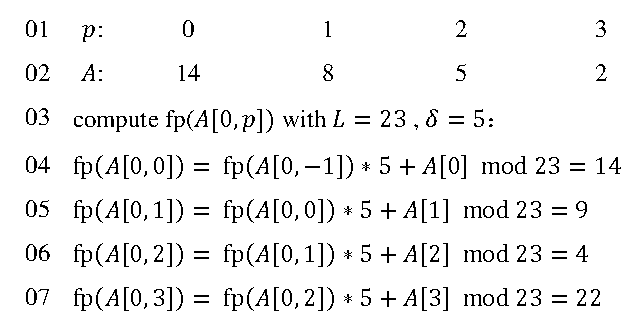
\includegraphics[width = 1\columnwidth]{example2.pdf}
	
	\caption{An example for calculating fingerprints by Karp-Rabin fingerprinting function.}
	
	\label{fig:example2}
	
\end{figure}

\subsection{Complexity Analysis}

<<<<<<< HEAD
Assuming the induction phase at the top recursion level is correctly implemented, the bottleneck of Algorithms~\ref{alg:2} and~\ref{alg:3} occur when checking $sa^*$. For Algorithm~\ref{alg:2}, we apply the method proposed in~\cite{wu2017} to ensure the correctness of $sa^*$ within the sorting complexity. Specifically, given two suffixes, i.e. ${\sf suf}(i)$ and ${\sf suf}(j)$, and their LCP-value $d$, we compute and compare the fingerprints of ${\sf sub}(i, i + d - 1)$ and ${\sf sub}(j, j + d - 1)$. If the fingerprints are equal and the order of $x[i + d]$ and $x[j + d]$ corresponds to that of ${\sf suf}(i)$ and ${\sf suf}(j)$, then the suffixes are correctly sorted and their LCP-value is right with a high probability. Because at most one out of every two suffixes is S*-type (commonly one-third in real-world data sets) and the checking process is only executed during the induction phase at the top recursion level, the checking overhead is much less than the building consumption. This conclusion is also true for Algorithm~\ref{alg:3}, where the checking overhead is mainly taken by computing fingerprints in need.
 
=======
The bottleneck of Algorithm~\ref{alg:2} and~\ref{alg:3} lie in checking the correctness of $sa^*$. For Algorithm~\ref{alg:2}, we apply the method proposed in~\cite{wu2017} to ensure the correctness of $sa^*$ within the sorting complexity. Specifically, given two suffixes, i.e. $\sf suf(i)$ and $\sf suf(j)$, and their LCP-value $d$, we compute and compare the fingerprints of $\sf sub(i, i + d - 1)$ and $\sf sub(j, j + d - 1)$. If the fingerprints are equal and the order of $x[i + d]$ and $x[j + d]$ corresponds to that of $\sf suf(i)$ and $\sf suf(j)$, then the suffixes are correctly sorted and their LCP-value is right with a high probability. Because at most one out of every two suffixes is S*-type (commonly one-third suffixes are S*-type in real-world data sets) and the checking process is only executed during the induction phase at the top recursion level, the checking overhead is much less than the building consumption. For Algorithm~\ref{alg:3}, the checking overhead is mainly caused by fingerprinting calculations and thus can be neglected compared with the building consumption.

>>>>>>> 72e840cf8c9fa565eba557b84e6beb4e2e547367
\section{Experiments} \label{sec:experiments}

For performance comparison, we engineer DSA-IS and DSA-IS+ by the STXXL's containers~(vector, sorter, priority queue and stream). The experimental platform is a desktop computer equipped with an Intel Xeon E3-1220 V2 CPU, 4GiB RAM and 500GiB HD. All the programs are complied by gcc/g++ 4.8.4 with -O3 options under Ubuntu 14.04 64-bit operating system. In our experiments, three performance metrics are investigated for the programs running on the corpora listed in Table~\ref{tbl:corpora}, where each metric is measured as a mean of two runs.

\begin{itemize}
	\item construction time~(CT): the running time, in units of microseconds per character.
	\item peak disk use~(PDU): the maximum disk space requirement, in units of bytes per character.
	\item I/O volume~(IOV): as the term suggests, in units of bytes per character.
\end{itemize}

%Table
\renewcommand\arraystretch{1.3}
\begin{table}[!h]
	\caption{Corpus, $n$ in Gi, 1 byte per character}
	\label{tbl:corpora}
	\centering
	\begin{tabular}{|l|c|c|p{5cm}|}
		\hline
		Corpora & \multicolumn{1}{c|}{$n$} & \multicolumn{1}{c|}{$\|\Sigma\|$} & Description \\\hline
		guten & 22.5 & 256 & Gutenberg, at \url{http://algo2.iti.kit.edu/bingmann/esais-corpus}.\\\hline 				
		enwiki & 74.7 & 256 & Enwiki, at \url{https://dumps.wikimedia.org/enwiki}, dated as 16/05/01. \\\hline	
		proteins & 1.1 & 27 & Swissprot database, at \url{http://pizzachili.dcc.uchile.cl/texts/protein}, dated as 06/12/15. \\\hline
		uniprot & 2.5 & 96 & UniProt Knowledgebase release 4.0, at \url{ftp://ftp.expasy.org/databases/.../complete}, dated as 16/05/11. \\\hline
	\end{tabular}
\end{table}

\subsection{Building Performance}

\begin{figure*}[t]
	\centering
	\subfigure[enwiki]{
		\begin{minipage}[b]{0.45\textwidth}
			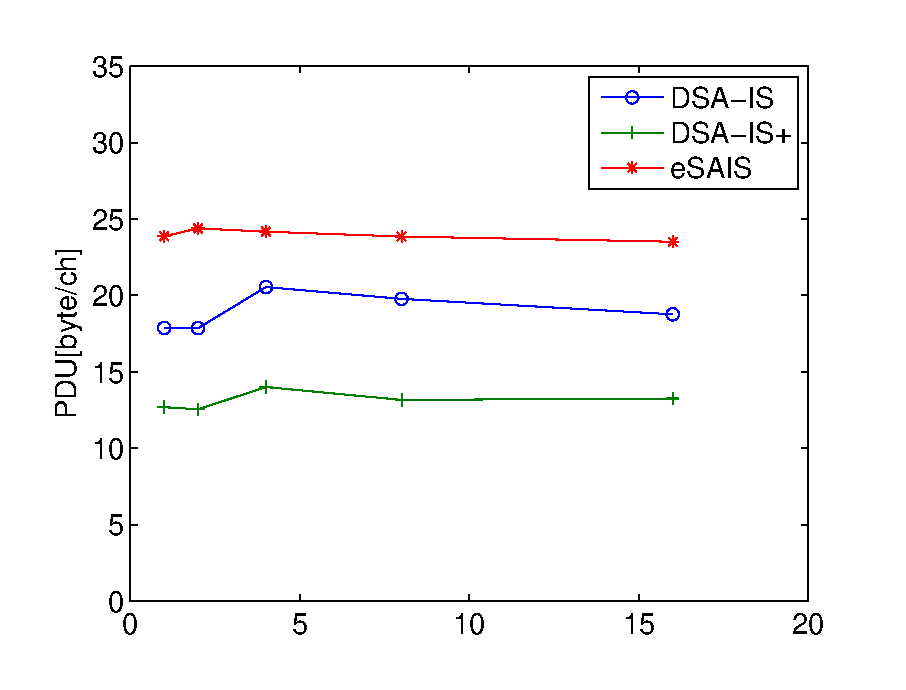
\includegraphics[width=1\textwidth]{construction_pdu_enwiki} \\
			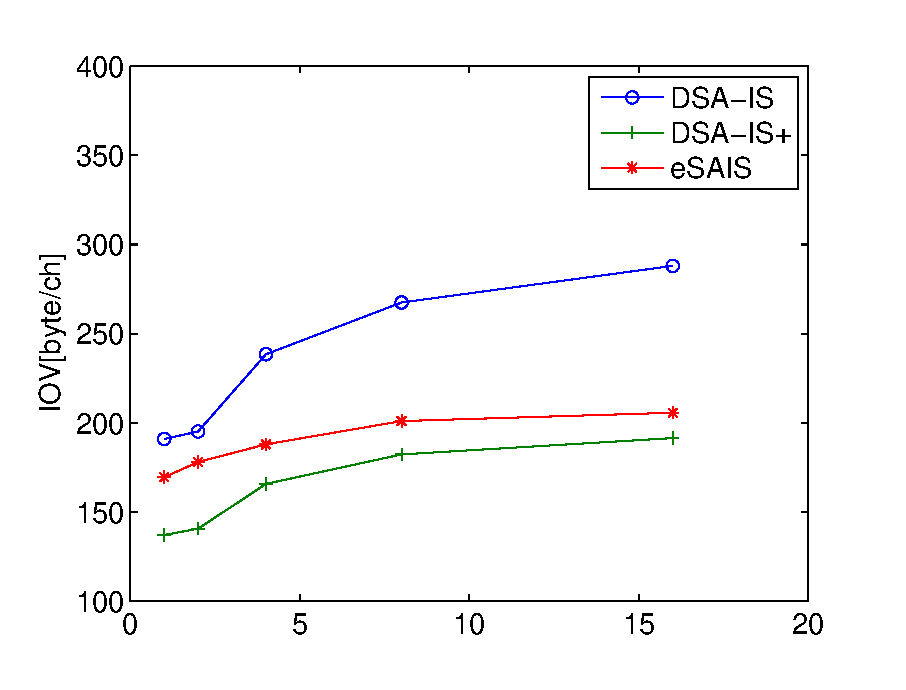
\includegraphics[width=1\textwidth]{construction_iov_enwiki} \\
			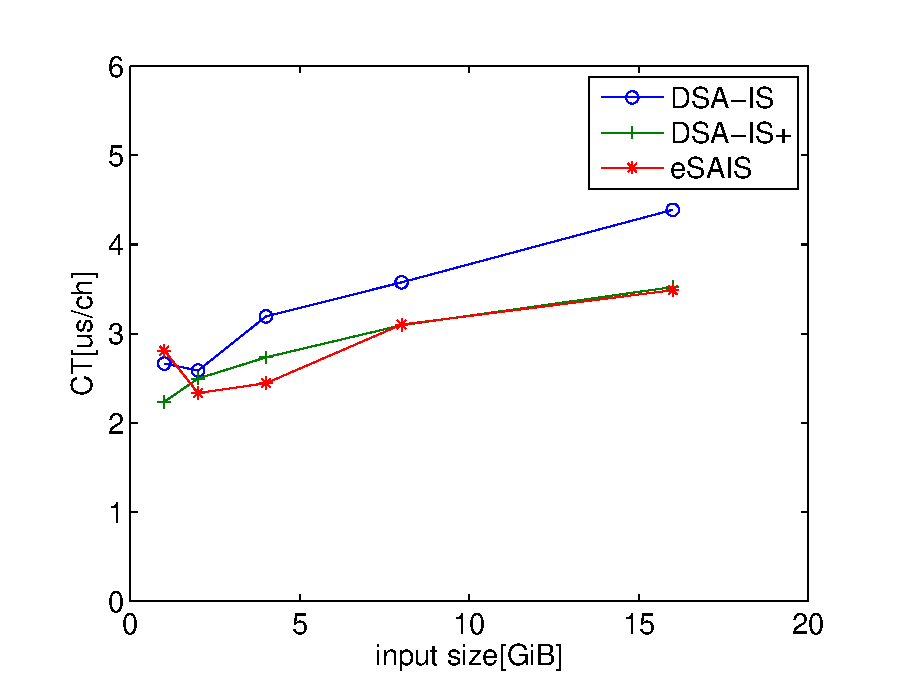
\includegraphics[width=1\textwidth]{construction_ct_enwiki}
		\end{minipage}
	}
	\subfigure[guten]{
		\begin{minipage}[b]{0.45\textwidth}
			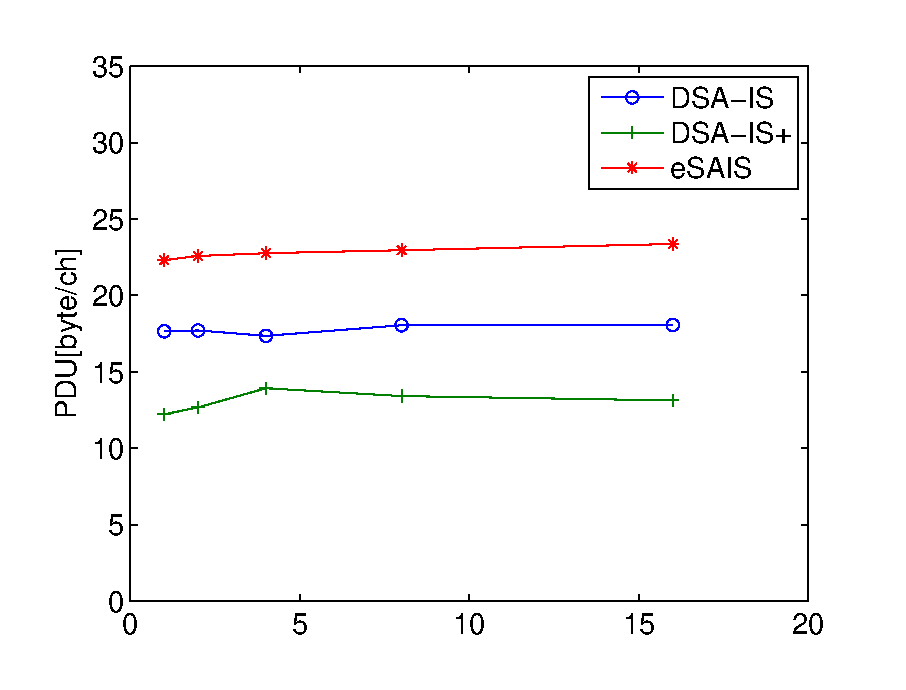
\includegraphics[width=1\textwidth]{construction_pdu_guten} \\
			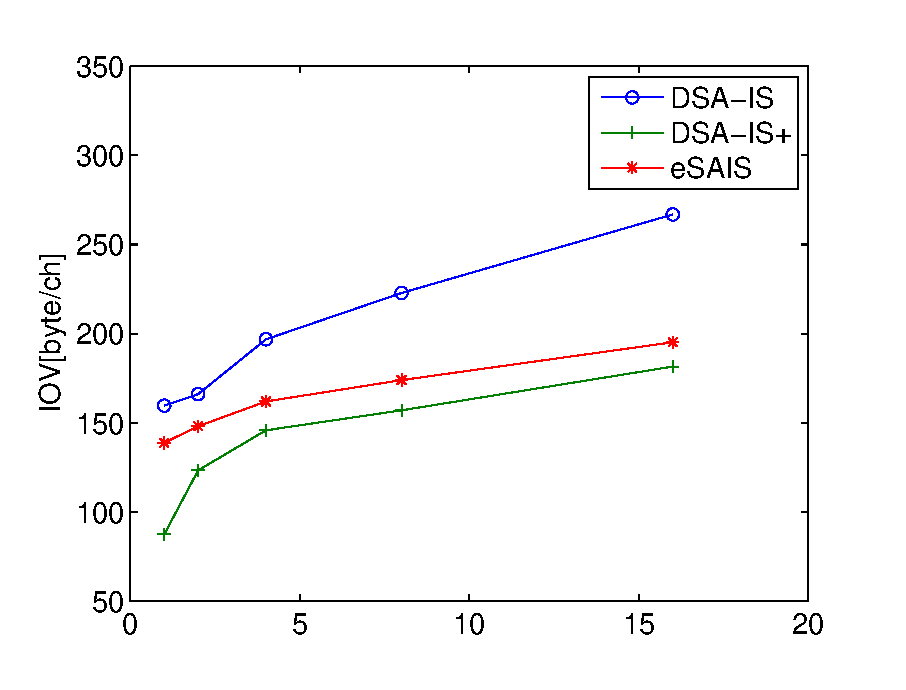
\includegraphics[width=1\textwidth]{construction_iov_guten} \\
			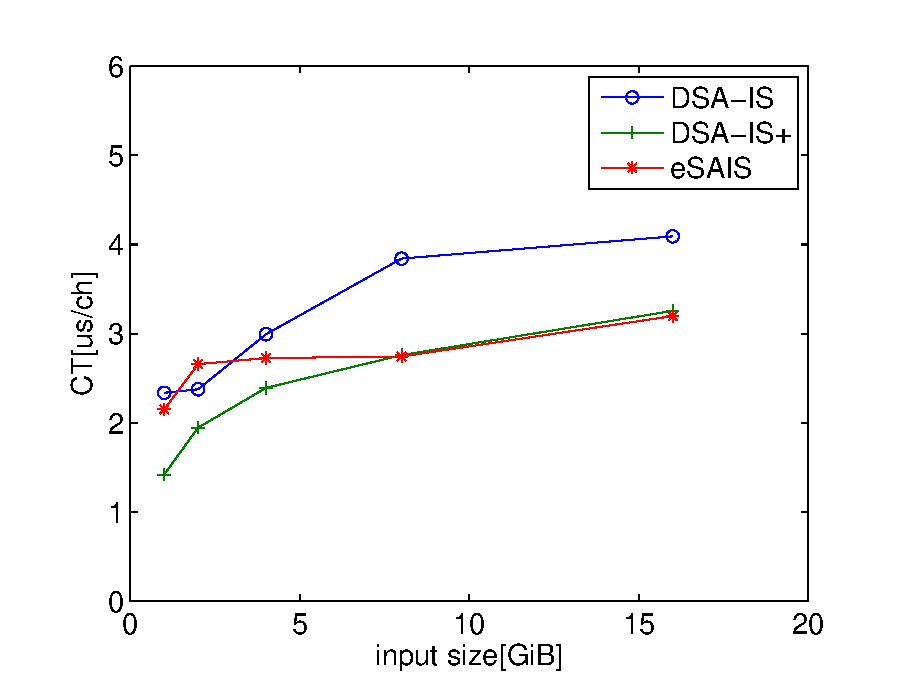
\includegraphics[width=1\textwidth]{construction_ct_guten}
		\end{minipage}
	}
	\caption{A comparison of DSA-IS, DSA-IS+ and eSAIS on guten and enwiki in terms of peak disk usage, I/O volume and construction time, where $D = 4$ and the input size varies in \{1, 2, 4, 8, 16\} GiB. }
	\label{fig:construction_performance1}
\end{figure*}

% Table
\begin{table*}%
	\caption{A Comparison of Reduction and Induction I/O Volumes Amongst DSA-IS, DSA-IS+ and eSAIS on enwiki}
	\label{tbl:volume_cmp}
	\centering
	\begin{tabular}{|c|c|c|c|c|c|c|c|c|c|c|c|c|}
		\hline
		\multicolumn{1}{|c}{} & \multicolumn{4}{|c|}{eSAIS} & \multicolumn{4}{c|}{DSA-IS} & \multicolumn{4}{c|}{DSA-IS+ ($D = 4$)}\\\hline
		\hline
		Size & Red. & Ind. & Total & Ratio & Red. & Ind. & Total & Ratio & Red. & Ind. & Total & Ratio\\\hline
		1G & 36.6 & 132.8 & 169.4 & 0.27 & 81.3 & 109.6 & 190.9 & 0.74 & 45.4 & 91.7 & 137.1 & 0.33\\\hline
		2G & 36.0 & 141.9 & 177.9 & 0.25 & 83.5 & 111.6 & 195.1 & 0.75 & 47.2 & 93.4 & 140.6 & 0.34\\\hline
		4G & 35.6 & 152.1 & 187.7 & 0.23 & 94.3 & 144.1 & 238.4 & 0.65 & 54.1 & 111.5  & 165.6 & 0.33\\\hline
		8G & 35.2 & 165.7 & 200.9 & 0.21 & 107.8 & 159.6 & 267.4 & 0.68 & 60.1 & 122.1 & 182.2 & 0.33\\\hline
		16G & 35.0 & 172.1 & 207.1 & 0.20 & 121.9 & 166.1 & 288.0 & 0.73 & 62.7 & 128.7 & 191.4 & 0.33\\\hline
	\end{tabular}
\end{table*}%

Because fSAIS is not available online, we use eSAIS as a baseline for analyzing the performance of DSA-IS and DSA-IS+, where the program for eSAIS is also implemented by the STXXL library. Fig.~\ref{fig:construction_performance1} shows a comparison between the programs for these three algorithms in terms of the investigated metrics. As depicted, the program for DSA-IS requires less disk space than that for eSAIS when running on "enwiki" and "guten". In details, the peak disk use of DSA-IS and eSAIS are around $18n$ and $24n$, respectively. However, eSAIS runs much faster than DSA-IS due to the different I/O volumes. In order for a deep insight, we collect in Table~\ref{tbl:volume_cmp} the statistics of their I/O volumes in the reduction and induction phases. As can be seen, although DSA-IS and eSAIS have similar performances when sorting suffixes in the induction phase, the latter consumes much less I/O volume than the former when sorting substrings in the reduction phase. More specifically, the mean ratio of induction I/O volume to reduction I/O volume are $0.23$ and $0.71$ for them, respectively. We can also see from the same figure that DSA-IS+ achieves a substantial improvement against DSA-IS, it runs as fast as eSAIS and takes half as much disk space as the latter. This is because the reduction I/O volume for DSA-IS+ is only half as much as that for DSA-IS (Table~\ref{tbl:volume_cmp}). Notice that the new substring sorting and naming methods adopted by DSA-IS+ take effect when most of the S*-type substrings are short. From our experiments, given $D = 8$, the ratio of long S*-type substrings in the investigated corpus nearly approaches one hundred percent, indicating that these methods are practical for real-world datasets.

\subsection{Checking Performance}

For evaluation, we integrate Method B into DSA-IS+ to constitute "Solution A" and compare it with "Solution B" composed of eSAIS and the existing checking method in~\cite{Dementiev2008a}. Fig.~\ref{fig:verification_performance} gives a glimpse of the performance of two solutions on various corpora. It can be observed that, the time, space and I/O volume for verification by Method B is negligible in comparison with that for construction by DSA-IS+, while the overhead for checking SA in Solution B is relatively large. Table~\ref{tbl:breakdown_solutionb} shows the performance breakdown of Solution B, where the checking time is one-fifth as the running time of the plain eSAIS and the peak disk use for verification is also a bit larger than that for construction. As a result, the combination of DSA-IS+ and Method B can build and check an SA in better total time and space.

\begin{figure}[t]
	\centering
	\subfigure{
		\label{subfig:verification_pdu}
		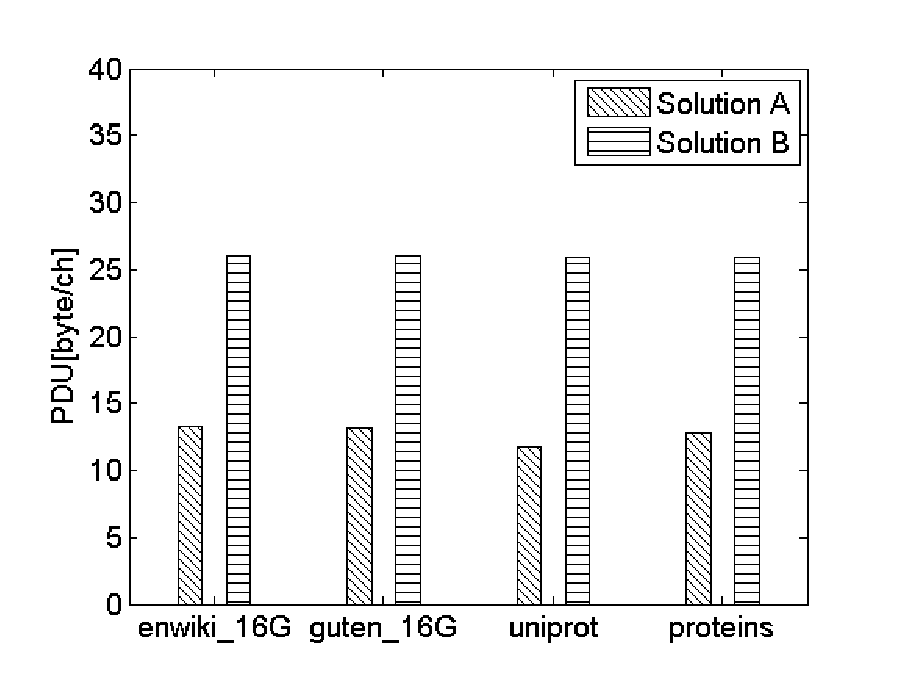
\includegraphics[width = 0.9\columnwidth]{verification_pdu}
	}
	\hfil
	\subfigure{
		\label{subfig:verification_iov}
		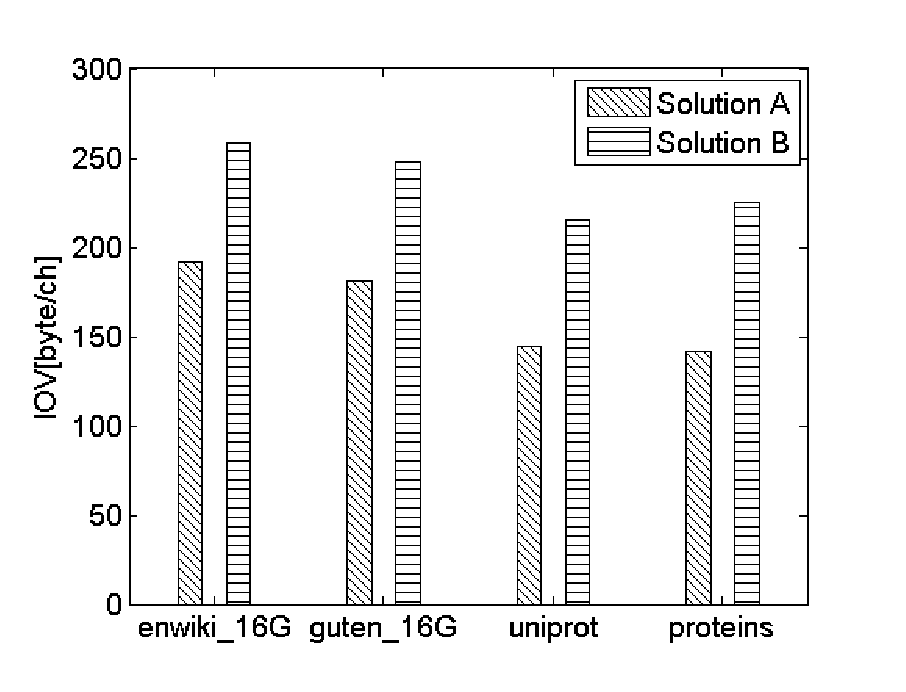
\includegraphics[width = 0.9\columnwidth]{verification_iov}
	}
	\hfil
	\subfigure{
		\label{subfig:verification_ct}
		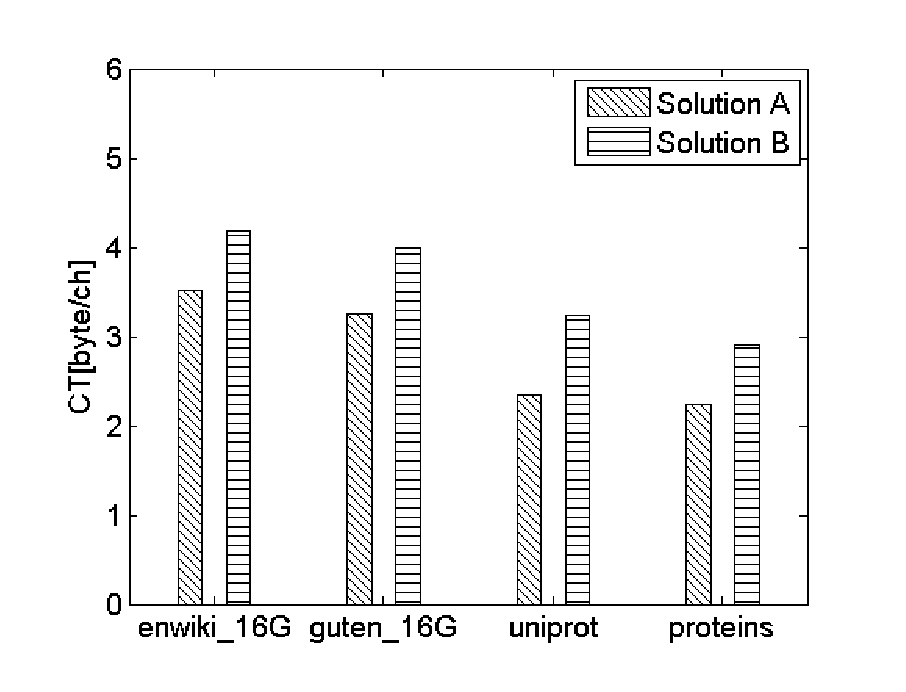
\includegraphics[width = 0.9\columnwidth]{verification_ct}
	}
	\caption{A comparison of Solutions A and B on various corpora in terms of peak disk usage, I/O volume and construction time, where $D = 4$.}
	\label{fig:verification_performance}
\end{figure}

% Table
\begin{table}%
	\caption{Performance Breakdown of Solution B on various Corpora}
	\label{tbl:breakdown_solutionb}
	\centering
	\begin{tabular}{|c|c|c|c|c|c|c|}
		\hline
		\multirow{2}{*}{Corpus} & \multicolumn{3}{|c}{checking} & \multicolumn{3}{|c|}{building} \\\cline{2-7}
		& PDU & IOV & CT & PDU & IOV & CT \\\hline
		enwiki\_16G & 26.0 & 53.0 & 0.71 & 23.5 & 205.6 & 3.49 \\\hline
		guten\_16G & 26.0 & 53.0 & 0.79 & 23.4 & 195.2 & 3.20 \\\hline
		uniprot & 25.9 & 53.0 & 0.74 & 22.7 & 162.0 & 2.50 \\\hline
		proteins & 25.9 & 53.0 & 0.58 & 24.1 & 172.3 & 2.33 \\\hline
	\end{tabular}
\end{table}%

\subsection{Discussion}

<<<<<<< HEAD
Rather than designing an I/O layer for efficient I/O operations, we currently use the containers provided by the STXXL library to perform reading, writing and sorting in external memory, these containers do not free the disk space for storing temporary data even if it is not needed any more, leading to a space consumption higher than our expectation. This is an implementation issue that can be solved by storing the data into multiple files and deleting each file when it is obsolete. In this way, our program can be further improved to achieve a space performance comparable to fSAIS. Our next paper will describe a novel disk-based IS suffix sorter that only takes 1n work space excluding the disk space for storing input and output. 

\section{Conclusion} \label{sec:conclusion}

By assuming the induction phase at the top recursion level is correctly implemented, we proposed two methods that enable any IS suffix sorter to build and check an SA simultaneously. The probabilistic algorithm designed by the second method is rather lightweight, it takes negligible time and space compared with the existing IS suffix sorting and checking algorithms. We also made our first attempt to improve the space performance of DSA-IS using new substring and naming methods. Our experimental results show that the program for the adapted algorithm DSA-IS+ runs as fast as that for eSAIS and consumes only half as much disk space as the latter on various real-world datasets. We are now designing and implementing a novel IS suffix sorter that takes no more than 1n work space on external memory model. Theoretically, this suffix sorter has a better space performance than fSAIS under the same circumstances. 
=======
Rather than designing an I/O layer for efficient I/O operations, we currently use the containers provided by the STXXL library to perform reading, writing and sorting in external memory, these containers do not free the disk space for storing temporary data even if it is not needed any more, leading to a space consumption higher than our expectation. This is an implementation issue that can be solved by storing the data into multiple files and deleting each file when it is obsolete. In this way, our program can be further improved to achieve a space performance comparable to fSAIS. In our next paper, we will propose another disk-based sorting algorithm that has a space performance even better than fSAIS. It takes only $1n$ work space to run excluding the input and output.

\section{Conclusion} \label{sec:conclusion}

We proposed two methods that enable any IS suffix sorting algorithm to build and check SA simultaneously. The program for our algorithm designed by Method B consumes negligible time and RAM space in comparison with that for the existing suffix sorting and checking algorithms on various real-world data sets. We also made our first attempt to improve the performance of DSA-IS using new substring and naming methods. The implementation for the adapted algorithm DSA-IS+ runs as fast as that for eSAIS and requires only half as much disk space as the latter. These results indicate the great potential of the IS method to design efficient solutions for SA constructing and verification. 

>>>>>>> 72e840cf8c9fa565eba557b84e6beb4e2e547367

\bibliographystyle{IEEEtran}
\bibliography{IEEEabrv,bibfile}

\end{document}
